\section{L04-Sistemi bifase}
\subsection{Sistema eterogeneo}
Un sistema \textbf{omogeneo} è un sistema con un solo stato di aggregazione.\newline
\newline
Un sistema \textbf{eterogeneo} è un sistema con più stati di aggregazione.\newline
\newline
Un sistema \textbf{monocomponente} è un sistema con una sola sostanza al suo interno.\newline
\newline
Un sisteam \textbf{multicomponente} è un sistea con più sostanze al suo interno.\newline
\newline
Le generica \textbf{grandezze estensive specifiche} $e$ di un sistema eterogeneo costituito da due stati di aggregazione $\alpha$ e $\beta$ possono essere rappresentate come \textbf{media pesata sulle masse} dei valori delle grandezze estensive specifiche delle singole fasi:
\[
    e = \frac{M_\alpha}{M}e_{\alpha} + \frac{M_\beta}{M}e_\beta
\]
\ \newline
Si definisce \textbf{frazione massica} le proporzioni di massa in uno stato di aggregazione rispetto alla massa complessiva. Per esempio in un generico sistema eterogeneo con due stati di aggregazione $\alpha$ e $\beta$:
\[
    x_\alpha = \frac{M_\alpha}{M} \;\;\;\;\;\;\;\;\;\;\;\;\;\;\; x_\beta = \frac{M_\beta}{M}
\]
Ricordiamo inoltre che 
\[
    x_\alpha + x_\beta = 1
\]
e che una generica grandezza estensiva specifica può quindi essere espressa come
\[
    e = x_\alpha e_\alpha + x_\beta e_\beta = (1-x_\beta)e_\alpha + x_\beta e_\beta
\]
\subsubsection{Regola di gibs per sistemi eterogenei}
\textbf{Regola di Gibbs}:
\[
    V = C + 2 -F
\]
$V$: numero di \textbf{variabili intensive indipendenti} utilizzabili per descrivere il generico stato di equilibrio.\newline
$C$: numero di componenti.\newline
$F$: numero di fasi.
\begin{itemize}
    \item Per il generico sistema \textbf{monocomponente e monofase} $V =2$, quindi per descrivere uno stato di equilibrio è sufficiente una coppia intensiva-intensiva (per esempio $P$ e $T$).
    \item Per il generico sistema \textbf{monocomponente bifase} $V =1$, quindi per descrivere lo stato termodinamico è necessaria una coppia intensiva-estensiva oppure un coppia estensiva-estensiva:\newline
    $(P,v) \;\; (T,v) \;\; (P,u) \;\; (T,u) \;\; (P,h) \;\; (T,h) \;\; (P,s) \;\; (T,s) \;\; (v,u) \;\; (v,h) \;\; (v,s) \;\; (u,h) \;\; (u,s) \;\; (h,s)$
    \item Per il generico sistema \textbf{monocomponente trifase} $V=0$, quindi per descirvere uno stato di equilibrio è necessaria un coppia estensiva-estensiva:\newline
    $(v,u) \;\; (v,h) \;\; (v,s) \;\; (u,h) \;\; (u,s) \;\; (h,s)$
\end{itemize}
\subsubsection{Transizione di fase}
Una \textbf{transizione di fase}:
\begin{itemize}
    \item è il passaggio da uno stato di aggregazione ad un altro;
    \item avviene a pressione (e temperatura) costatne.
\end{itemize}
\ \newline
Definiamo l'\textbf{entalpia di transizione} come la quantità di energia necessaria per passare da uno stato a un altro:
\[
    dh = \delta q^\leftarrow 
\]
\subsubsection{Sistemi eterogenei monocomponente}
Possibili configurazioni:
\begin{itemize}
    \item \textbf{Stati monofase}:
    \begin{itemize}
        \item Solido
        \item Liquido 
        \item Aeriforme (Gas)
    \end{itemize}
    \item \textbf{Stati bifase}:
    \begin{itemize}
        \item Coesistenza di solido e liquido
        \item Coesistenza di solido e aeriforme (vapore)
        \item Coesistenza di liquido e aeriforme (vapore)
    \end{itemize}
    \item \textbf{Stati tripli}:
    \begin{itemize}
        \item Coesistenza di solido, liquido e aeriforme (vapore)
    \end{itemize}
\end{itemize}
Terminologia:
\begin{itemize}
    \item \textbf{Liquido sottoraffreddato}: liquido non in porcinto di evaporare (temperatura di sistema sotto temperatura di saturazione)
    \item \textbf{Liquido saturo}: liquido in procinto di evaporare (liquido a temperatura di saturazione)
    \item \textbf{Vapore saturo}: vapore in condizioni di incipiente condensazione (gas a temperatura di saturazione)
    \item \textbf{Vapore surriscaldato}: vapore non in procinto di condensare (temperatura di sistema sopra temperatura di saturazione)
    \item \textbf{Temperatura di saturazione}: temperatura alla quale una sostanza pura comincia ad evaporare (se è un liquido) oppure condensare (se è un gas), fissata la pressione.
\end{itemize}
\subsection{Diagramma di stato P-v-T}
\subsubsection{terminologia}
\begin{center}
    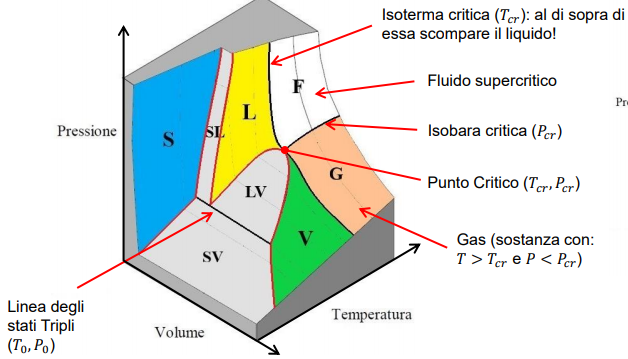
\includegraphics[height=5cm]{../L04/img2.PNG}
\end{center}
\begin{center}
    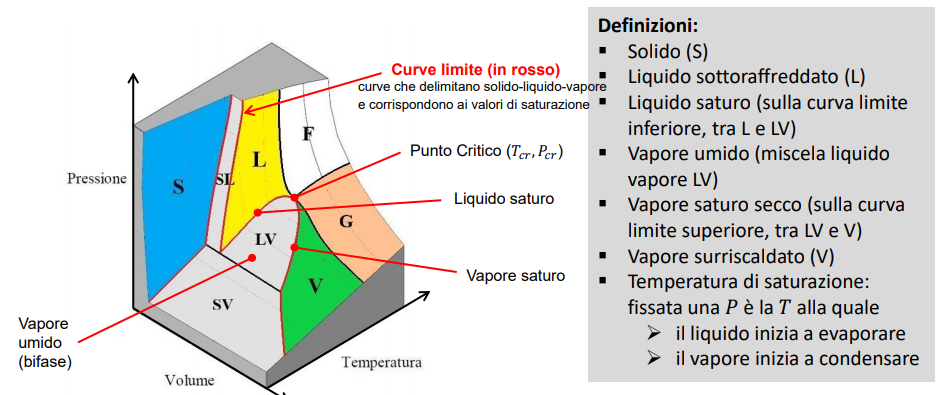
\includegraphics[height=5cm]{../L04/img1.PNG}
\end{center}
\subsubsection{Proiezione del diagramma P-v-T in un grafico P-T}
\begin{center}
    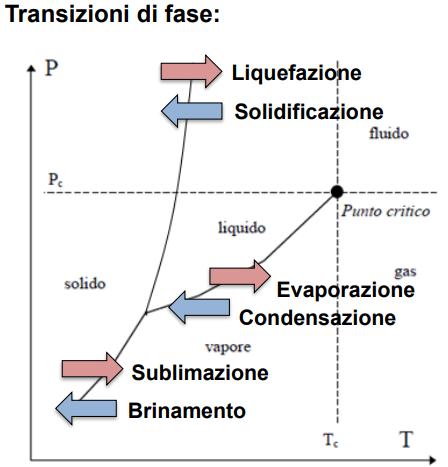
\includegraphics[height=7cm]{../L04/img3.PNG}
\end{center}
\subsubsection{Gas}
Fluido a $P< P_{cr}$ e $T> T_{cr}$ che non può essere liquefatto attraverso una trasformazione di compressione isoterma:
\begin{center}
    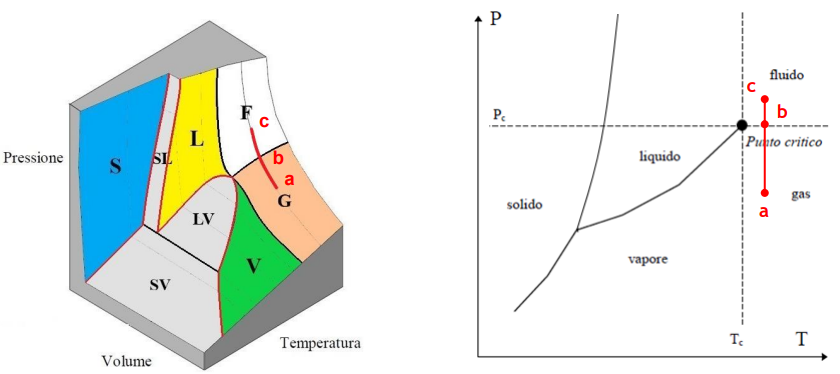
\includegraphics[height=7cm]{../L04/img4.PNG}
\end{center}
\subsubsection{Trasformazione isobara}
\begin{center}
    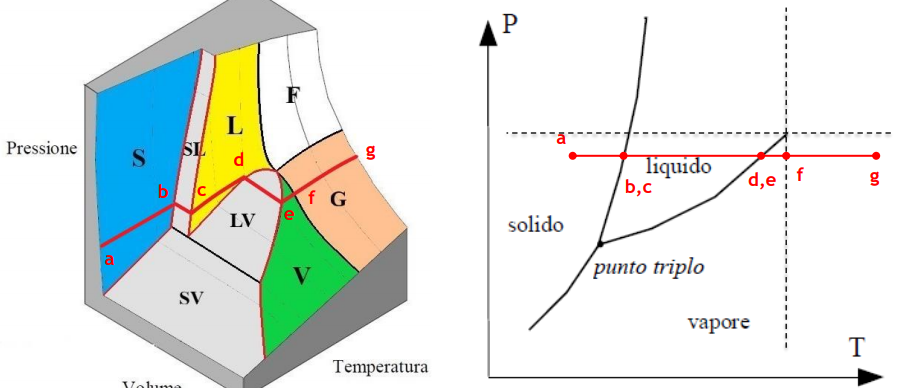
\includegraphics[height=6cm]{../L04/img6.PNG}
\end{center}
\begin{center}
    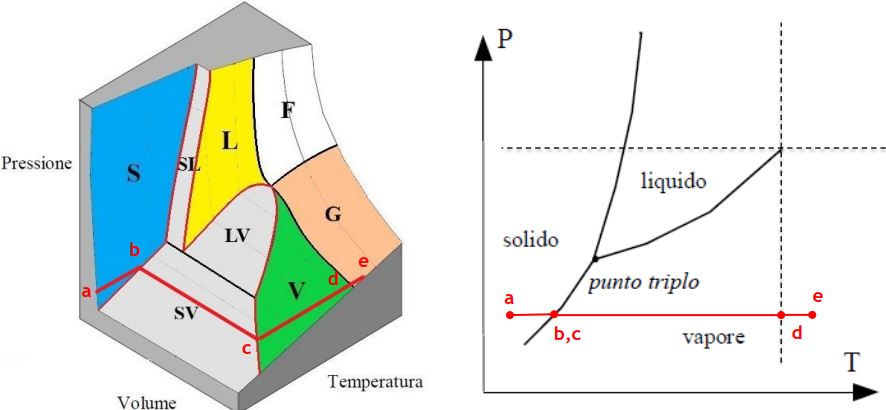
\includegraphics[height=7cm]{../L04/img5.PNG}
\end{center}
\subsubsection{Traformazione isoterma}
\begin{center}
    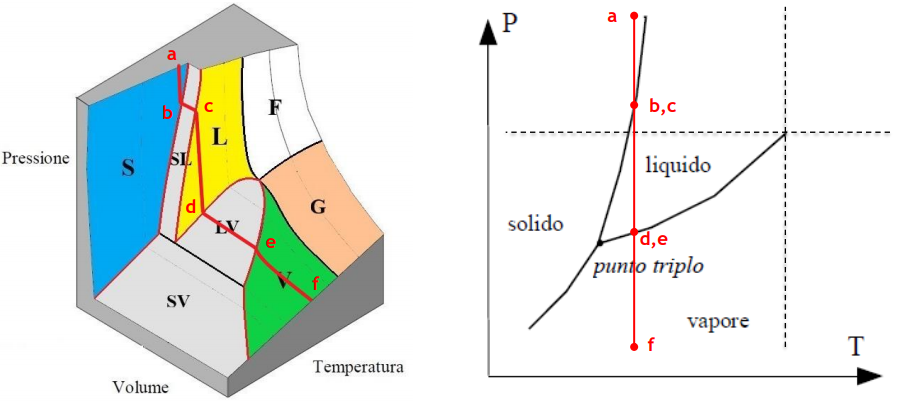
\includegraphics[height=6cm]{../L04/img7.PNG}
\end{center}
\subsubsection{Proiezione del diagramma P-v-T in un grafico P-s e P-h}
Uno dei problemi del proiettare la superficie di stato ne ldiagramm $P-T$, è che difficilmente riusciamo a rappresentare le transizioni di fase, perchè, per esempio le zone SL e LV corrispondono soltanto a un punto. Perciò il diagramma $P-T$ è poco utili per rappresentare i cambi di stato. Per ovviare a ciò dobbiamo fare diverse proiezioni della superficie di stato, rispetto a una coppia di grandezze $(P,v)$, per esempio:
\begin{center}
    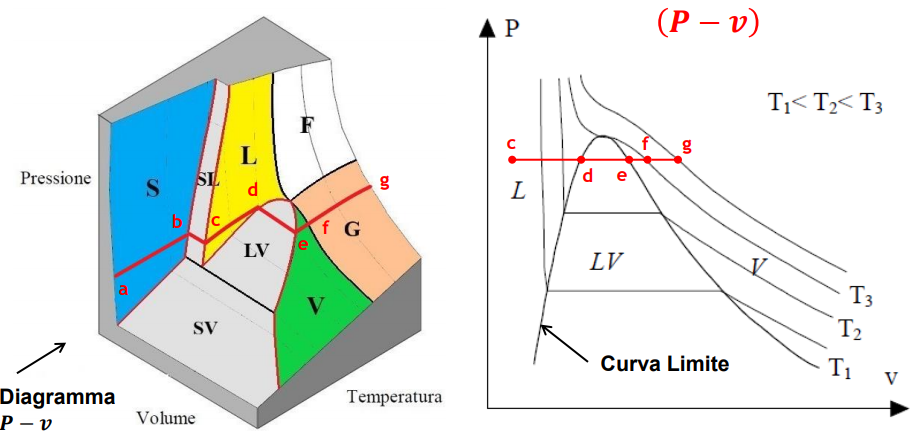
\includegraphics[height=6cm]{../L04/img8.PNG}
\end{center}
Una soluzione a questo problema di rappresentazion è l'utilizzo del diagramma temperatura-entropia, per esempio:
\begin{center}
    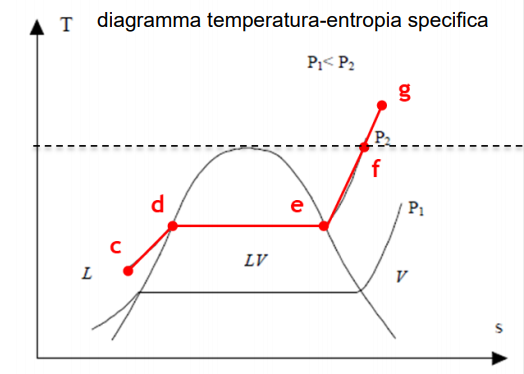
\includegraphics[height=6cm]{../L04/img9.PNG}
\end{center}
Il tipo di diagramma utilizzato varia a seconda dello scopo che si vuole raggiungere, ce ne sono anche molti altri, per esempio quello $P-h$ e quello $h-s$.
\subsection{Proprietà termodinamiche dei sistemi eterogenei}
\subsubsection{Entalpia di transizione di fase}
\[
    h_{solido} < h_{liquido} < h_{vapore}
\]
\begin{itemize}
    \item entalpia di \textbf{liquefazione}: $h_{liquido}-h_{solido} > 0$
    \item entalpia di \textbf{solidificazione}: $h_{lst}= h_{solido}- h_{liquido} < 0$
    \item entalpia di \textbf{evaporazione}: $h_{lvt} = h_{vapore}- h_{liquido} >0$
    \item entalpia di \textbf{condensazione}: $h_{liquido}-h_{vapore} <0$
    \item entalpia di \textbf{sublimazione}: $h_{svt} = h_{vapore}- h_{solido} >0$
    \item entalpia di \textbf{brinamento}: $h_{solido}-h_{vapore} <0$
\end{itemize}
\subsubsection{Titoli}
Le frazioni massiche dei tre stati di aggregazione prendono il nome di \textbf{titolo}:
\begin{itemize}
    \item \textbf{titolo di vapore}: $x_v = \frac{M_v}{M}$
    \item \textbf{titolo di liquido}: $x_l = \frac{M_l}{M}$
    \item \textbf{titolo di solido}: $x_s = \frac{M_s}{M}$
\end{itemize}
Ricordiamo che $x_v + x_l + x_s = 1$ e che una generica \textbf{grandezza estensiva} $e$ può essere espressa come:
\[
    e = (1-x_l-x_v) e_s + x_l e_l + x_v e_v
\]
\subsection{Tabelle termodinamiche}
\subsubsection{Tabella di saturazione in pressione}
E' detta "in pressione" perchè sulla prima colonna sono indicate le \textbf{pressioni}.\newline
La seconda colonna rappresenta delle \textbf{temperature}.\newline
\newline
La prima riga è sempre quella che rappresenta il \textbf{punto triplo}.\newline
\newline
Ogni coppia di valori Pressione-Temperatura presente in tabella segue la \textbf{curva di saturazione liquido-vapore} proiettata su un diagramma $P-T$.\newline
\newline
Per ogni coppia $P-T$ specificato in tabella sono indicati i seguenti valori:
\begin{itemize}
    \item \textbf{volume specifico} (terza, quarta, quinta colonna)
    \item \textbf{entalpia specifica} (sesta, settima, ottava colonna)
    \item \textbf{entropia specifica} (nona, decima, undicesima colonna)
\end{itemize}
Per ognuno di questi valori viene indicato il valore per \textbf{liquido saturo}, per \textbf{vapore saturo} e la differenza fra questi ultimi due.
\begin{center}
    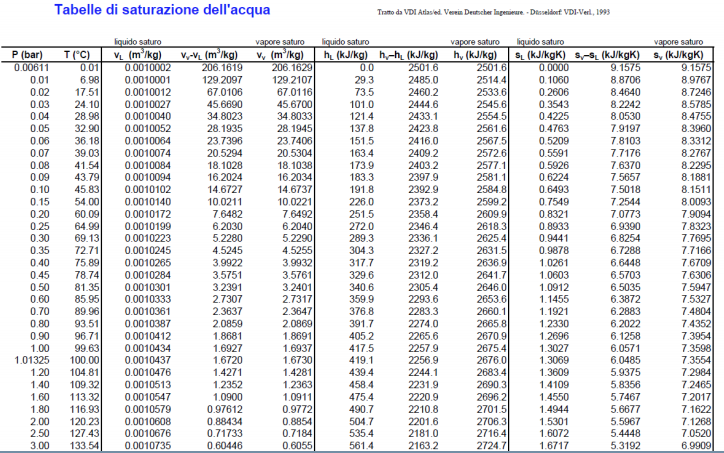
\includegraphics[height=7cm]{../L04/img10.PNG}
\end{center}
\subsubsection{Tabella di saturazione in temperatura}
E' detta "in temperatura" perchè sulla prima colonna sono indicate le \textbf{temperature}.\newline
La seconda colonna rappresenta delle \textbf{pressioni}.\newline
\newline
Il contenuto della tabella è il medesimo della tabella precedente, solo che il riferimento è basato sulla temperatura (sono in ordine di temperatura) e non sulla pressione.
\begin{center}
    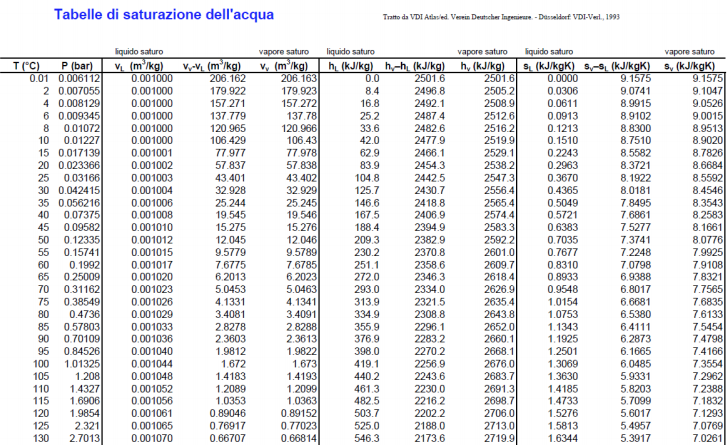
\includegraphics[height=7cm]{../L04/img11.PNG}
\end{center}
\subsubsection{Tabella del vapore surriscaldato}
Questa tabella mostra le pressioni sulle righe e le temperature sulle colonne, per un sistema monofase, in cui $P$ e $T$ descrivono uno stato di equilibrio.\newline
\newline
Per ogni riga di pressione, è mostrata la \textbf{temperatura} $T_s$ di \textbf{saturazione} a tale pressione.\newline
\newline
Per ogni coppia temperatura - pressione che andiamo a cercare  troviamo i valori di \textbf{volume specifico}, \textbf{entalpia specifica}, \textbf{entropia specifica}.\newline
\newline
La zona evidenziata in giallo, senza valori, rappresentano i valori oltre la curva limite, cioè la zona di liquido sottoraffreddato, dove $T_s > T$.
\begin{center}
    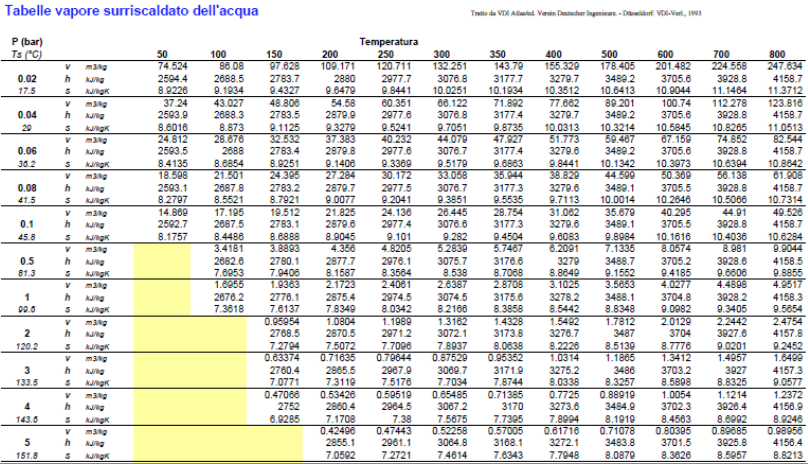
\includegraphics[height=7cm]{../L04/img12.PNG}
\end{center}
\subsubsection{Interpolazione lineare}
Siccome non è possibile creare tabelle con ogni possibile valore, per tutti quei casi in cui non si trova una corrispondenza precisa nella tabella, si usa lì \textbf{interpolazione lineare}
\[
    Y = Y_A + \frac{Y_B - Y_A}{X_B - X_A}(X - X_A)
\]
$Y$: grandezza che si vuole ricavare.\newline
$X$: grandezza conosciuta.\newline
$A,B$: stati di riferimento (presenti in tabella) con $X_A < X < X_B$.
\subsubsection{interpolazione bilineare}
Nel caso in cui più di una grandezza non corrisponda a nessun valore preciso della tabella usiamo la formula di \textbf{interpolazione bilineare}
\[
    Y = Y_A + \frac{Y_B - Y_A}{X_B - X_A}(X - X_A)
\]
\[
    Y_A = Y_{A1} + \frac{Y_{A2}- Y_{A1}}{X_{A2}- X_{A1}} (X_A - X_{A1})
\]
\[
    Y_B = Y_{B1} + \frac{Y_{B2}- Y_{B1}}{X_{B2}- X_{B1}} (X_B - X_{B1})
\]
\subsubsection{Formule per l'acqua sottoraffreddata}
Vediamo come calcolare tutti quei valori per cui non esistono tabelle, per esempio i valori per un liquido sottoraffreddato.\newline
\newline
\textbf{Modello di liquido incomprimibile ideale}\newline
Per un liquido incomprimibile ideale abbiamo $c_P = c(T), \beta = 0, K_T = 0$ e
\[
    dh = c(T) dT + v dP
\]
\[
    ds = c(T) \frac{dT}{T}
\]
che sono forme differenziali e per poterle integrare devo conoscere la funzione $c(T)$, che però non conosciamo. L'ipotesi che quindi facciamo è quella di liquido incomprimibile perfetto, cioè con $c$ costante.\newline
\newline
\textbf{Modello di liquido incomprimibile perfetto}\newline
Per un liquido incomprimibile perfetto abbiamo $c = costaten$ e quindi possiamo integrare le formule viste precedentemente e otteniamo
\[
    \Delta h = c\Delta T + v \Delta P
\]
\[
    \Delta s = c ln \frac{T_2}{T_1}
\]
Dalla prima di queste due formule posso scrivere che
\[
    h - h_{ref} = c(T-T_{ref}) + v (P-P_{ref})
\]
dove col pedice "ref" si intendono valori che troviamo in tabella per liquidi saturi.\newline
\newline
Possiamo ora procedere in due maniere: fissando la temperatura (corretto) o fissando la pressione (sbagliato).\newline
\newline
\textbf{Approccio a temperatura costante}:
\begin{center}
    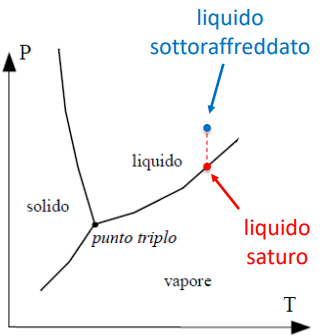
\includegraphics[height=5cm]{../L04/img13.PNG}
\end{center}
La situazione è questa: stiamo cercando di calcolare il punto azzurro di "liquido sottoraffreddato" usando le tabelle di liquido saturo che ci permettono di individuare il punto rosso di "liquido saturo" alla medesima temperatura.
\newline
sostituiamo i valori con pedice "ref" dell'equazione precedentemente trovata
\[
    h - h_{ref} = c(T-T_{ref}) + v (P-P_{ref})
\]
con i valori che troviamo con la tabella di liquido saturo eccetto per la temperatura che teniamo fissa:
\[
    h(P,T) - h_{ls}(P_{sat}(T)) = c(T - T) + v (P - P_{sat}(T))
\]
\[
    h(P,T) = h_{ls} (P_{sat}(T)) + v (P-P_{sat}(T))
\]
inoltre per $v$ si può usare il valore del liquido saturo fornito dalla tabella $v = v_{ls}(P_{sat}(T))$.\newline
\newline
\textbf{Approccio a pressione costante}:\newline
\textbf{N.B. non usare questo approccio!}
\begin{center}
    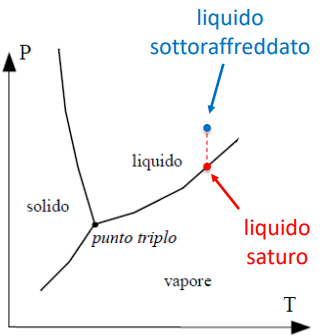
\includegraphics[height=5cm]{../L04/img13.PNG}
\end{center}
La situazione è questa: stiamo cercando di calcolare il punto verde di "liquido sottoraffreddato" usando le tabelle di liquido saturo che ci permettono di individuare il punto rosso di "liquido saturo" alla medesima pressione.\newline
Se seguiamo il medesimo procedimento di prima ma con pressione fissa, otteniamo:
\[
    h(P,T) - h_{ls}(T_{sat}(P)) = c (T-T_{sat}(P)) + v(P-P)
\]
\[
    h(P,T) = h_{ls}(P_{sat} (T)) + c (T-T_{sat}(P))
\]
che non è valido perchè in genere $c \neq costante$.\newline
Cosa fare se si conosce $P$ e non $T$? (TODO, vedi esercizio ES 3.1.6)\newline
\newline
\textbf{Caso nel quale si conosce (P,h) e si vuole conoscere T}\newline
\[
    h(P,T) = h_{ls}(P_{sat}(T)) + v(P-P_{sat}(T))
\]
in cui solitamente $v (P-P_{sat}(T))$ è solitamente trascurabile, e dunque si interpola in tabella di saturazione la temperatura per la quale $h_{ls}(T) = h$.\newline
\newline
\textbf{Caso nel quale si conosce (P,s) e si vuole conoscere T}\newline
Approccio simile a quello precedente.
\subsection{Relazioni semplificate vicino al punto triplo per l'acqua}
In assenza di tabelle, si possono usare le seguenti relazioni semplificate che rimandono valide in prossimità \textbf{punto triplo} per lo stato solido, lo stato liquido e lo stato vapore.
\begin{center}
    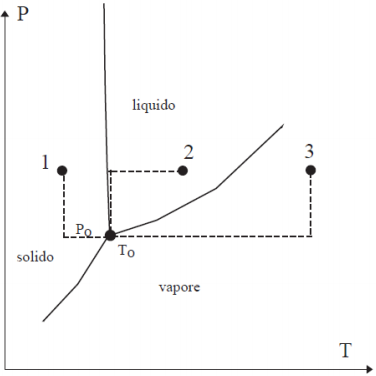
\includegraphics[height=5cm]{../L04/img15.PNG}
\end{center}
\subsubsection{Stato solido}
\[
    h(P,T) = h_0 + h_{lst} + c_s(T-T_0) + v_s(P-P_0)
\]
\[
    s(P,T) = s_0 +s_{lst} + c_s ln \frac{T}{T_0} = s_0 + \frac{h_{lst}}{T_0} + c_s ln \frac{T}{T_0}
\]
con \newline
$P_0, T_0$: pressione e temperatura del punto triplo ($P_0 = 0,00611 bar ; T_0 = 0.01 C^o$)\newline
$h_0$: entalpia di riferimento al punto triplo in fase liquida ($h_0 = 0 kJ/kg$)\newline
$s_0$: entropia di riferimento al punto triplo in fase liquida ($s_0 = 0kJ/kgK$)\newline
$h_{lst}$: entalpia di solidificazione al punto triplo ($h_{lst} = -333 kJ/kg$)\newline
$c_s$: calore specifico del ghiaccio ($c_s = 2093 J/kgK$)\newline
$v_s$: volume specifico del ghiaccio ($v_s = 0.00109 m^3/kg$)\newline
Possiamo approssimare $T_{sat, L-S}(P) = T_0$.
\subsubsection{Stato liquido}
(USARE LE TABELLE)
\[
    h(P,T) = h_0 + c_{l}(T-T_0) + v_l (P-P_0)
\]
\[
    s(P,T) = s_0 + c_l ln \frac{T}{T_0}
\]
con \newline
$P_0, T_0$: pressione e temperatura del punto triplo ($P_0 = 0,00611 bar ; T_0 = 0.01 C^o$)\newline
$h_0$: entalpia di riferimento al punto triplo in fase liquida ($h_0 = 0 kJ/kg$)\newline
$s_0$: entropia di riferimento al punto triplo in fase liquida ($s_0 = 0kJ/kgK$)\newline
$c_{l}$: calore specifico dell'acqua liquida ($c_l = 4186 J/kgK$)\newline
$v_{l}$: volume specifico dell'acqua liquida ($v_l = 0,001 m^s/kg$)
\subsubsection{Stato vapore}
(USARE LE TABELLE)
\[
    h(P,T) = h_0 + h_{lvt} + c_p (T-T_0)
\]
\[
    s(P,T) = s_0 + s_{lvt} + c_p ln \frac{T}{T_0} - R^* ln \frac{P}{P_0} = s_0 + \frac{h_{lvt}}{T_0} c_P ln \frac{T}{T_0}- R^* ln \frac{P}{P_0}
\]
con \newline
$P_0, T_0$: pressione e temperatura del punto triplo ($P_0 = 0,00611 bar ; T_0 = 0.01 C^o$)\newline
$h_0$: entalpia di riferimento al punto triplo in fase liquida ($h_0 = 0 kJ/kg$)\newline
$s_0$: entropia di riferimento al punto triplo in fase liquida ($s_0 = 0kJ/kgK$)\newline
$h_{lvt}$: entalpia di evaporazione al punto triplo ($h_{lvt} = 2501.6 kJ/kg$)\newline
$c_P$: calore specifico a pressione costante dell'acqua vapore ($c_P = 2009 J/kgK$)